\hypertarget{programme}{%
\section{Programme}\label{programme}}

\begin{itemize}
\tightlist
\item
  Frameworks MVC : Laravel, Django, \ldots{}
\item
  HTML5 : vue d'ensemble
\item
  Javascript : VueJS, Node.js, jQuery, AJAX, JSON, \ldots{}
\item
  Déploiement et configuration Serveur
\item
  Webservices : REST vs SOAP
\item
  Sécurité : Technologies, prévention des risques courants
\item
  (Responsive) Web Design
\item
  (Syndication : RSS, Atom)
\item
  {Vos souhaits ?}
\end{itemize}

\hypertarget{contenu-activituxe9s}{%
\section{Contenu, activités}\label{contenu-activituxe9s}}

\begin{itemize}
\tightlist
\item
  Cours théorique
\item
  2 Projets

  \begin{itemize}
  \tightlist
  \item
    frameworks : Laravel, Django, Vue.js (ouvert à d'autres
    propositions)
  \item
    Groupes de 3, \href{https://www.he-arc.ch/reglementation}{30h} par
    personne et par projet
  \item
    Présentation de 20min
  \end{itemize}
\item
  Workshops intervenants externes

  \begin{itemize}
  \tightlist
  \item
    Webdesign (\href{https://www.alinekeller.ch}{A. Keller}) ?
  \item
    Flask (\href{http://www.matthieuamiguet.ch/}{M. Amiguet}) ?
  \item
    Automatisation du déploiement
    (\href{https://www.linkedin.com/in/raphaelemourgeon/}{R. Emourgeon})
    ?
  \item
    {Vos présentations ? Vos propositions ?}
  \end{itemize}
\item
  Support : \href{https://he-arc.github.io/slides-devweb/}{ghpages}
  (\href{https://github.com/HE-Arc/slides-devweb/tree/master/src}{source}),
  partage fichiers :
  \href{https://teams.microsoft.com/l/team/19\%3ahGPvEcXl8HCohGre1MLq7AQ4qPWNkY_JqMTTPMPLM-I1\%40thread.tacv2/conversations?groupId=cadc33cc-9fc8-49d7-b951-aa26d534e15f\&tenantId=5b3b7d7d-e119-4d05-9022-f775f2e48e96}{teams}
\end{itemize}

\hypertarget{projets}{%
\section{Projets}\label{projets}}

\begin{itemize}
\tightlist
\item
  Faire pour apprendre
\item
  Les rôles dans une équipe de développement web, workflow
\item
  Ne pas réinventer la roue ou tout faire soi-même
\item
  Critères d'évaluation d'un projet
\item
  En profiter pour apprendre des choses qui vous intéressent
\item
  Avant le 1er octobre :

  \begin{itemize}
  \tightlist
  \item
    Avoir un compte github avec une
    \href{https://github.com/settings/keys}{clé SSH} (indispensable au
    déploiement)
  \item
    Constitution des équipes de 3 personnes
  \item
    Choix du projet
  \item
    Forge : Créer projet sur github dans l'entité
    \href{https://github.com/HE-Arc/}{HE-Arc}
  \item
    \href{https://github.com/HE-Arc/slides-devweb/wiki/Projets-2022-2023}{S'inscrire}
  \end{itemize}
\end{itemize}

\hypertarget{choix-des-projets}{%
\section{Choix des projets}\label{choix-des-projets}}

\begin{itemize}
\tightlist
\item
  Contrainte : appli basée sur des données
\item
  Choix

  \begin{itemize}
  \tightlist
  \item
    Besoin réel
  \item
    Données existantes : \href{http://wiki.dbpedia.org/}{dbpedia},
    \href{https://opendata.swiss/fr/}{opendata}, \ldots{}
  \item
    S'inspirer de l'existant :

    \begin{itemize}
    \tightlist
    \item
      \href{https://www.producthunt.com/topics/web-app}{Product Hunt},
      \href{http://www.makeuseof.com/tag/best-websites-internet/}{makeuseof},
      \ldots{}
    \item
      \href{https://github.com/HE-Arc/}{Volées précédentes}
    \end{itemize}
  \end{itemize}
\item
  Commencer tôt pour se libérer les dernières semaines de l'année
\end{itemize}

\hypertarget{calendrier}{%
\section{Calendrier}\label{calendrier}}

\begin{longtable}[]{@{}rlrl@{}}
\toprule
Semaine & Automne & Semaine & Printemps\tabularnewline
\midrule
\endhead
38 & Projet PHP & 8 &\tabularnewline
39 & & 9 &\tabularnewline
40 & & 10 & Rendu intermédiaire\tabularnewline
41 & S. thématique & 11 &\tabularnewline
42 & & 12 &\tabularnewline
43 & & 13 &\tabularnewline
44 & Rendu intermédiaire & 14 &\tabularnewline
45 & & 16 &\tabularnewline
46 & & 17 &\tabularnewline
48 & & 18 & Présentations\tabularnewline
49 & & 19 & Présentations\tabularnewline
50 & & 20 & Examens\tabularnewline
51 & Présentations & 21 & Début TB\tabularnewline
2 & Projet Python & &\tabularnewline
3 & & &\tabularnewline
4 & & &\tabularnewline
5 & T. Autonome & &\tabularnewline
6 & Examen & &\tabularnewline
\bottomrule
\end{longtable}

\hypertarget{suivi-du-calendrier-uxe0-jour-sur-teamsteams}{%
\section{\texorpdfstring{Suivi du calendrier (à jour sur
\href{https://teams.microsoft.com/l/team/19\%3ahGPvEcXl8HCohGre1MLq7AQ4qPWNkY_JqMTTPMPLM-I1\%40thread.tacv2/conversations?groupId=cadc33cc-9fc8-49d7-b951-aa26d534e15f\&tenantId=5b3b7d7d-e119-4d05-9022-f775f2e48e96}{teams})}{Suivi du calendrier (à jour sur teams)}}\label{suivi-du-calendrier-uxe0-jour-sur-teamsteams}}

\begin{figure}
\centering
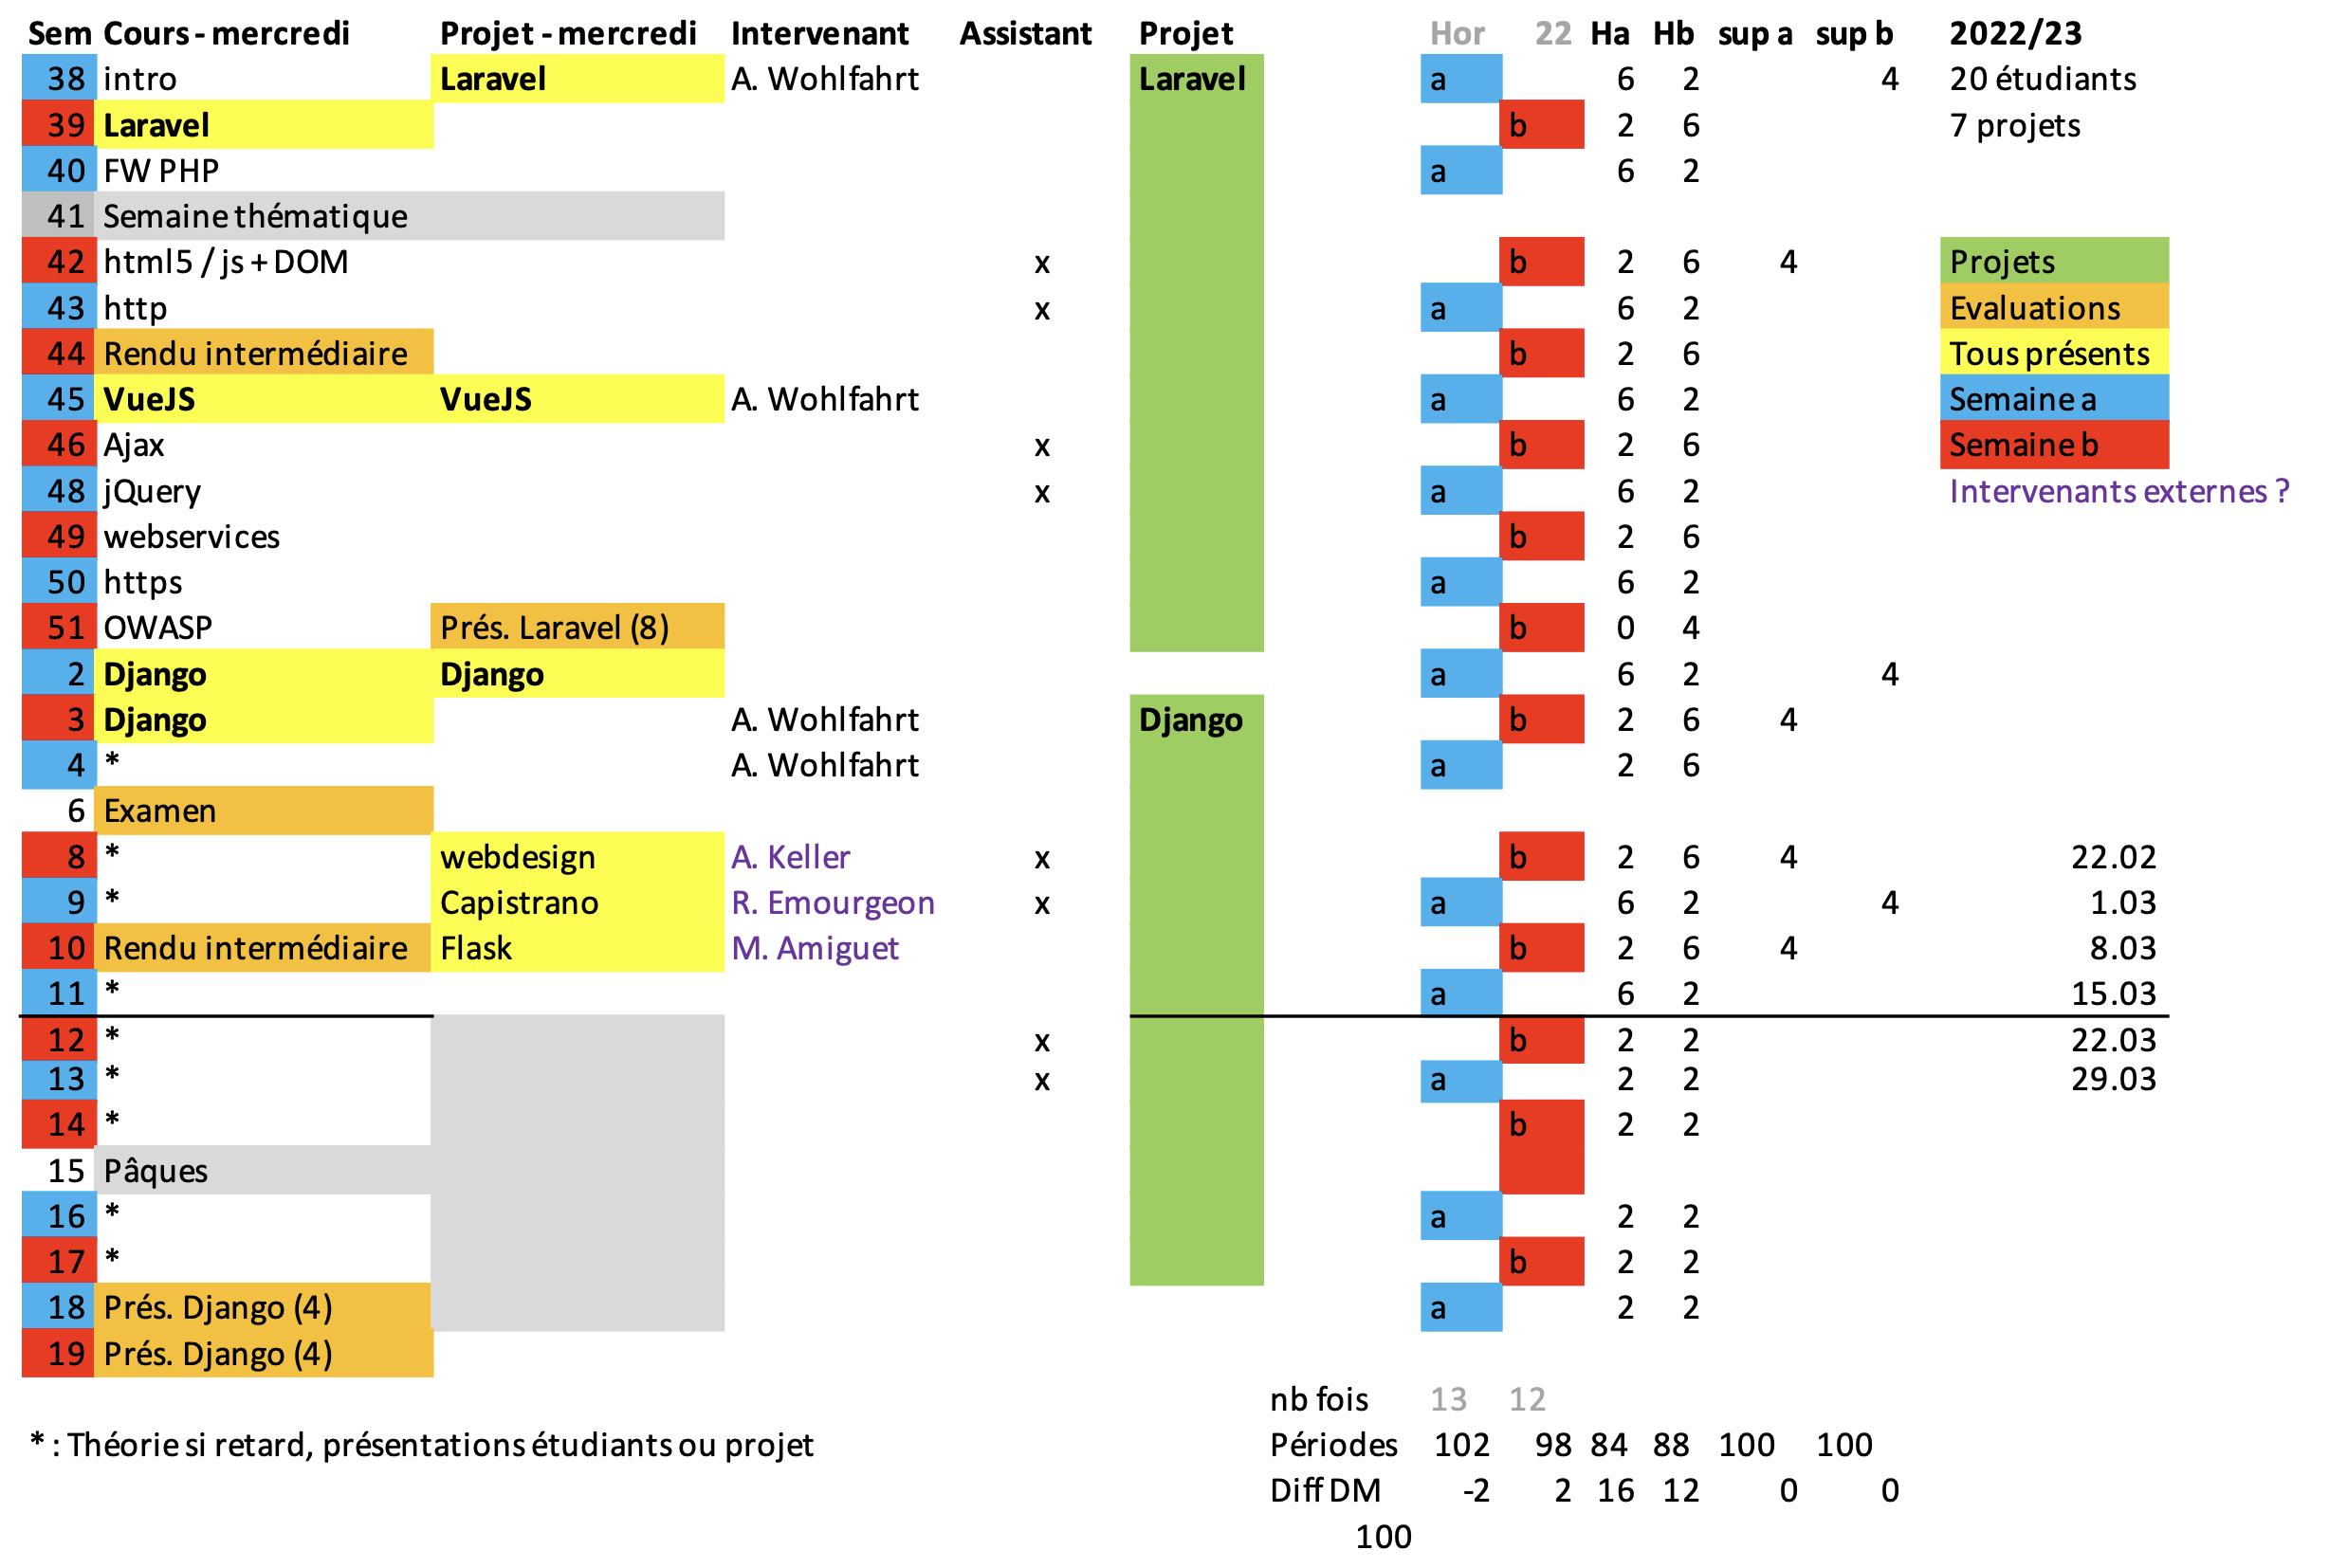
\includegraphics{src/img/DW2223.png}
\caption{Suivi calendrier}
\end{figure}

\hypertarget{jalons-pour-chacun-des-2-projets}{%
\section{Jalons pour chacun des 2
projets}\label{jalons-pour-chacun-des-2-projets}}

\begin{itemize}
\tightlist
\item
  Echéances

  \begin{itemize}
  \tightlist
  \item
    En début de semaine, pour chacun des projets :

    \begin{enumerate}
    \def\labelenumi{\arabic{enumi}.}
    \tightlist
    \item
      Formation équipe et choix thème
    \item
      Objectifs et maquettes
    \item
      Authentification et 1er déploiement
    \item
      Modèles avec relations (au moins 3, dont 1 n-n)
    \item
    \item
      {Rendu intermédiaire (1x {[}route, validation, contrôleur, vue{]}
      GET et POST + bonne pratique Laravel + app déployé)}
    \item
    \item
      Minimal Viable Product
    \item
    \item
    \item
    \item
      {Rendu projet, Présentation}
    \end{enumerate}
  \end{itemize}
\item
  Il n'est pas interdit d'en ajouter
\end{itemize}

\hypertarget{conseils}{%
\section{Conseils}\label{conseils}}

\begin{itemize}
\tightlist
\item
  Le plus simple possible, pas trop de données
\item
  Application crédible (vraies données, cas réalistes)
\item
  Projet à blanc pour la prise en main du framework
\item
  \href{https://brainhub.eu/blog/difference-between-wireframe-mockup-prototype/}{Maquettes}
\item
  \href{http://drewfradette.ca/a-simpler-successful-git-branching-model/}{Organisez}
  l'utilisation du dépôt
\item
  Le temps disponible à l'horaire ne suffira pas !
\item
  Essayez de commit avec la même identité
\item
  Signalez dans le commit msg si vous n'êtes pas l'auteur
\item
  Le déploiement est long : commencez tôt !
\item
  Il est moins risqué travailler plus au début du projet qu'à la fin !
\item
  Discutez ! Echangez !
\end{itemize}

\hypertarget{uxe9valuation-des-projets}{%
\section{Évaluation des projets}\label{uxe9valuation-des-projets}}

\begin{itemize}
\tightlist
\item
  Note intermédiaire :

  \begin{itemize}
  \tightlist
  \item
    1 page permettant d'afficher des données provenant de la BDD

    \begin{itemize}
    \tightlist
    \item
      p.ex. : Liste de tous les utilisateurs
    \end{itemize}
  \item
    1 page permettant d'enregistrer des données dans la BDD

    \begin{itemize}
    \tightlist
    \item
      p.ex. : Création d'un utilisateur
    \end{itemize}
  \item
    Respect des conventions et bonnes pratiques
  \item
    Respect du pattern MVC : Les requêtes doivent passer par toutes les
    étapes importantes de Laravel

    \begin{itemize}
    \tightlist
    \item
      route, validation des entrées, contrôleur, vue
    \end{itemize}
  \item
    Application déployée avec tous les éléments cités plus haut testable
    et fonctionnel
  \item
    UI/UX peut donner des bonus

    \begin{itemize}
    \tightlist
    \item
      Mais la note sera focalisée sur l'aspect fonctionnel de
      l'application
    \item
      Et le code
    \end{itemize}
  \end{itemize}
\end{itemize}

\hypertarget{uxe9valuation-des-projets---suite}{%
\section{Évaluation des projets -
suite}\label{uxe9valuation-des-projets---suite}}

\begin{itemize}
\tightlist
\item
  Note finale :

  \begin{itemize}
  \tightlist
  \item
    Code : 50\%

    \begin{itemize}
    \tightlist
    \item
      Absence bugs, qualité code, lisibilité, respect conventions et
      bonnes pratiques
    \item
      Déploiement, configuration
    \end{itemize}
  \item
    User Experience : 30\%

    \begin{itemize}
    \tightlist
    \item
      Design UI, Utilisabilité (Efficacité, efficience, satisfaction)
    \end{itemize}
  \item
    Gestion de projet : 20\%

    \begin{itemize}
    \tightlist
    \item
      Fichiers versionnés, messages de commit, Issues, planification,
      travail en équipe
    \item
      Documentation (wiki), Investissement, volume de travail
    \end{itemize}
  \item
    Bonus (ceux qui vont plus loin) : 0-20\%

    \begin{itemize}
    \tightlist
    \item
      WebSockets ou autre API HTML5, webservices, \ldots{}
    \item
      Contribution, présentation, documentation, \ldots{}
    \end{itemize}
  \end{itemize}
\item
  {Tous les membres d'un groupe n'ont pas forcément la même note}
\end{itemize}

\hypertarget{participation}{%
\section{Participation}\label{participation}}

\begin{itemize}
\tightlist
\item
  Aux projets des autres : Issues, PR
\item
  Participez à la
  \href{https://hacktoberfest.digitalocean.com/}{Hacktoberfest}
\item
  Pariticipez au cours : contenu, présentation, pages
  (\href{https://he-arc.github.io/}{index},
  \href{https://github.com/HE-Arc/slides-devweb/wiki}{wiki}, \ldots)
\item
  Echangez avec \href{https://caravel.ing.he-arc.ch/}{caravel} (groupes
  : 22-ISC3il-a et 22-ISC3il-b) et tout autre im (discord, teams,
  \ldots)
\end{itemize}

\hypertarget{pruxe9sentation-facultative}{%
\section{Présentation facultative}\label{pruxe9sentation-facultative}}

\begin{itemize}
\tightlist
\item
  Facultatif, ne peut qu'augmenter la moyenne
\item
  DOIT être annoncé au semestre d'automne
\item
  Un thème absent du cours
\item
  2 à 4 personnes
\item
  Une présentation claire avec démo (printemps)
\item
  Un exercice d'application
\item
  Critiques et discussion
\item
  Au plus tôt :

  \begin{itemize}
  \tightlist
  \item
    Constitution des équipes
  \item
    Proposer 1 à 3 thèmes
  \item
    \href{https://docs.google.com/spreadsheet/viewform?formkey=dEVJRE1WVTVPelhFcE94TGF5N1c0cGc6MQ}{Proposer}
    le(s) thème(s) de présentation et l'équipe
  \end{itemize}
\end{itemize}

\hypertarget{examen-oral-sa}{%
\section{Examen oral SA}\label{examen-oral-sa}}

\begin{itemize}
\tightlist
\item
  Généralités pour la partie dev web de l'examen :

  \begin{itemize}
  \tightlist
  \item
    Vous n'avez droit à rien : on vous mettra à disposition 1 crayon et
    du papier pour préparer votre présentation,
  \item
    L'examen porte sur toute la matière vue au en cours (yc workshops),
  \item
    Les questions sont générales, il s'agit de présenter des concepts
    vus en cours (souvent 1 chapitre), et expliquer certains mécanismes
    sous-jacents,
  \item
    Il n'agit pas de réciter le contenu des slides par coeur, mais de
    les présenter avec vos propres mots (compréhension), et vos propres
    exemples.
  \end{itemize}
\end{itemize}

\hypertarget{examen-oral-sa-1}{%
\section{Examen oral SA}\label{examen-oral-sa-1}}

\begin{itemize}
\tightlist
\item
  Déroulement :

  \begin{itemize}
  \tightlist
  \item
    Vous tirez un n° de question au hasard pour chaque cours
  \item
    Vous disposez de 15 min pour préparer une présentation de 10 min
    pour chacun des 2 cours (pendant la présentation de l'étudiant
    précédent)
  \item
    Idéalement vous faites une présentation d'environ 10 min et les 5
    min restantes sont dédiées aux questions (pour chacun des cours)
  \end{itemize}
\end{itemize}

\hypertarget{mon-expuxe9rience-en-duxe9veloppement-web}{%
\section{Mon expérience en développement
web}\label{mon-expuxe9rience-en-duxe9veloppement-web}}

\begin{itemize}
\tightlist
\item
  \href{https://docs.google.com/spreadsheet/viewform?formkey=dDg5Znh5akRBV1hPbC1qYlVRV3BONFE6MQ}{Questionnaire}
  obligatoire (votre username github vous y sera demandé)
\end{itemize}

\hypertarget{section}{%
\subsubsection{🙏 !}\label{section}}

\hypertarget{sources}{%
\section{Sources}\label{sources}}
